%@def.tex
\documentclass[landscape]{slides}
\usepackage[warn]{mathtext}
\usepackage[T2A]{fontenc}
\usepackage[utf8]{inputenc}
\usepackage[english, russian]{babel}
\usepackage{indentfirst}
\usepackage{amsmath, amsfonts, amssymb}
\usepackage{geometry}
\usepackage{hyperref}
\usepackage{wrapfig}
\geometry{top=2cm}
\geometry{left=3cm}
\geometry{right=2cm}
\geometry{bottom=2cm}
\usepackage{color}
\usepackage{multirow}
\usepackage{lscape}
\usepackage{wrapfig}
\usepackage{graphicx}
\usepackage{epstopdf}
\usepackage{tikz}
\usepackage{tikz-3dplot}
\usetikzlibrary{arrows}
\usetikzlibrary{calc}

\renewcommand{\vec}{\overline}
\renewcommand{\phi}{\varphi}

\graphicspath{{pics/}}

\makeatletter
\newcommand{\nextverbatimspread}[1]{%
    \def\verbatim@font{%
        \linespread{#1}\normalfont\ttfamily% Updated definition
            \gdef\verbatim@font{\normalfont\ttfamily}}% Revert to old definition
}
\makeatother

\newenvironment{mintemize}{%
    \vspace{-1.5em}
    \begin{itemize}
        \setlength\itemsep{-0.2em}
}
{
    \end{itemize}
    \vspace{-1em}
}

\newenvironment{cslide}{%
    \begin{slide}
    \begin{center}
}
{
    \end{center}
    \end{slide}
}

\makeatletter
\def\sltop{\let\@topfil\relax}
\makeatother

\newenvironment{tslide}[1]{%
    \begin{slide}
    \sltop
    {\large\textbf{#1}}
}
{ \end{slide} }


\graphicspath{{pics/}}

\newenvironment{mintemize}%
{
    \vspace{-1.5em}
    \begin{itemize}
        \setlength\itemsep{-0.2em}
}
{
    \end{itemize}
    \vspace{-1em}
}

\newenvironment{cslide}
{
    \begin{slide}
    \begin{center}
}
{
    \end{center}
    \end{slide}
}

\begin{document}

\begin{cslide}
    
\includegraphics[width=4cm]{mai.eps}

    \textbf{ Разработка алгоритмов управления
    массивом беспилотных летательных аппаратов
    с целью построения информационного поля
    участка местности}

    \vspace{4em}

    \begin{flushright}
    \small Выполнил студент гр. 07-608 Бутко О.А.

    \small Руководитель Жидков В.Н.
    \end{flushright}

    \vspace{2em}

    \small Москва, 2014

\end{cslide}

\begin{slide}

    \makeatletter
    \let\@topfil\relax
    \makeatother

    \textbf{Постановка задачи}

    Разработать алгоритмы управления
    массивом беспилотных летательных аппаратов
    с целью построения информационного поля
    участка урбанистической местности.

    Требуется разработать модель массива летательных аппаратов,
    карту участка местности, построить алгоритмы сбора и доступа
    к информации, построить алгоритмы перемещния ЛА на основе собранной
    информации, а так же с учётом других ЛА массива,
    разработать симулятор для отлаживания деталей алгоритмов.
\end{slide}

\begin{slide}

    \makeatletter
    \let\@topfil\relax
    \makeatother

    \textbf{Актуальность проблемы}

    Всё чаще возникает проблема ведения боевых действий
    в черте города. В связи с этим растёт необходимость в технических
    решениях, которые позволят быстро и безопасно разведать местность.
    Массив миниатюрных и дешёвых БПЛА может справится с этой задачей 
    лучше как никто другой. Так же, такой массив может решать задачи недоступные
    для решения с помощью классических беспилотников для наблюдения, а именно: 
    \begin{mintemize}
        \item построение трёхмерной динамической карты местности
        \item исследование помещений
        \item непрерывный трекинг подвижных объектов
    \end{mintemize}

    Так же к плюсам такой системы можно отнести высокую робастность в плане
    устойчивости к потерям едениц, так как количество едениц в массиве
    практически не ограниченно, а потеря даже 90\% массива не сможет
    вывести систему из строя до конца.  Качество решаемой задачи
    будет плавно падать с падением количества едениц массива.
\end{slide}

\begin{slide}

    \makeatletter
    \let\@topfil\relax
    \makeatother

    \textbf{Решение задачи в рамках преддипломной работы}

    Основой частью работы можно считать программное обеспечение для моделирования
    массива. Главными проблемами являлись построение карты и отображение процесса работы системы
    в реальном времени. Решением этих двух задач является использование гетерогенных 
    вычислений с интероперабельностью с графикой. Были применены распостранённые 
    технологии такие как \verb|OpenGL| и \verb|OpenCL|.

    \begin{flushleft}
        
\includegraphics[width=0.4\linewidth]{opengl.png}
    \end{flushleft}

    \hfill

    \vspace{-9em}
    \begin{flushright}
    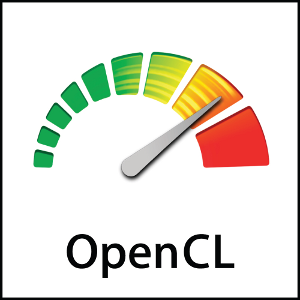
\includegraphics[width=0.3\linewidth]{opencl.png}
    \end{flushright}

\end{slide}

\begin{slide}

    \makeatletter
    \let\@topfil\relax
    \makeatother

    \textbf{Модель карты местности}

    Предполагается что участок местности ограничен по ширине, глубине и высоте.
    Он разбивается на прямоугольные сектора, каждый из которых хранит информацию об единице объёма местности:
    \begin{mintemize}
        \item был ли сектор исследован
        \item содержится ли в секторе что-либо
    \end{mintemize}

    Реализация карты представляет собой 1-мерный массив, к которому можно обратиться с помощью трёх
    индексов-координат. Так же для карты имеется матрица трансформации координат из локальных (индексов)
    в глобальные (метры).

    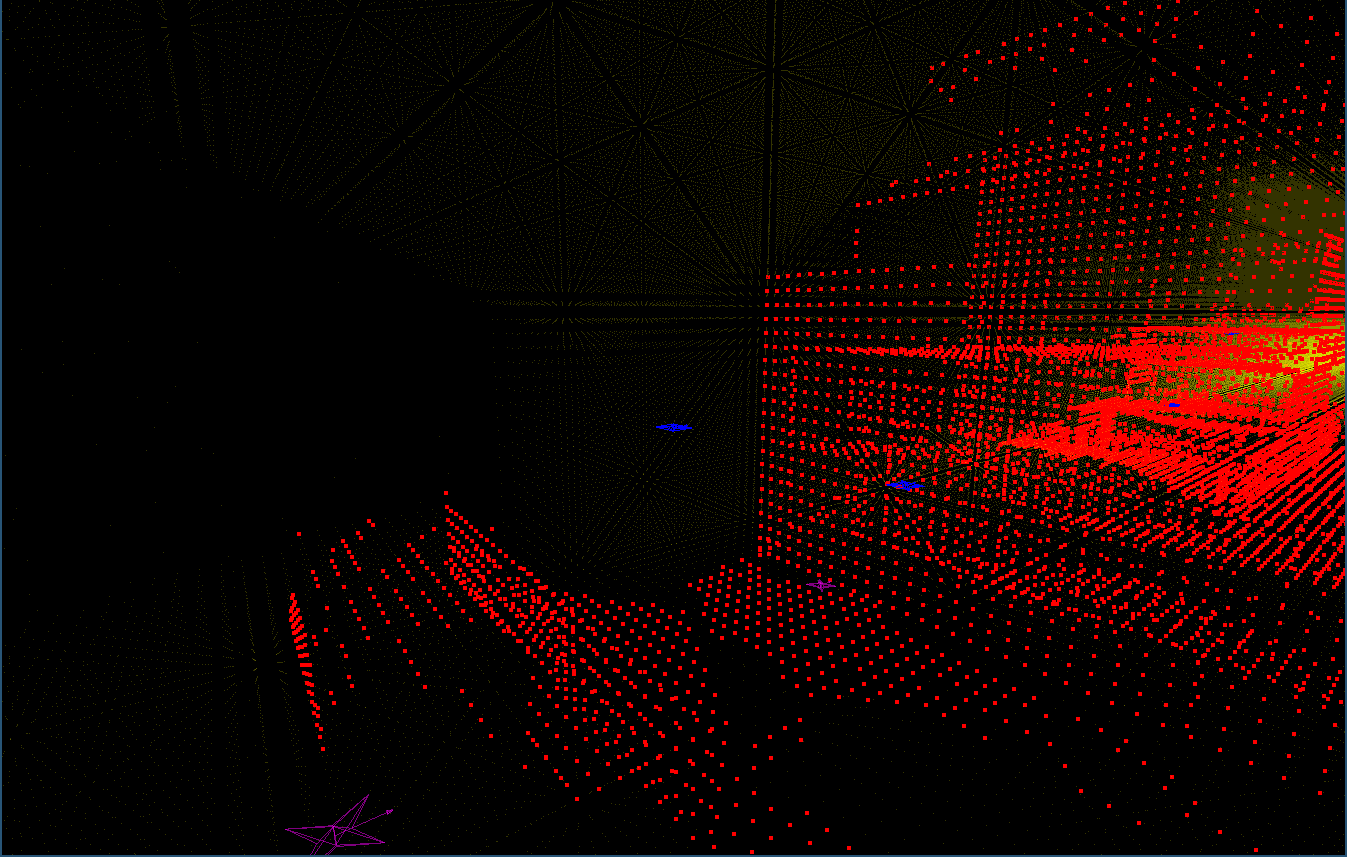
\includegraphics[width=0.33\linewidth]{map1.png}
    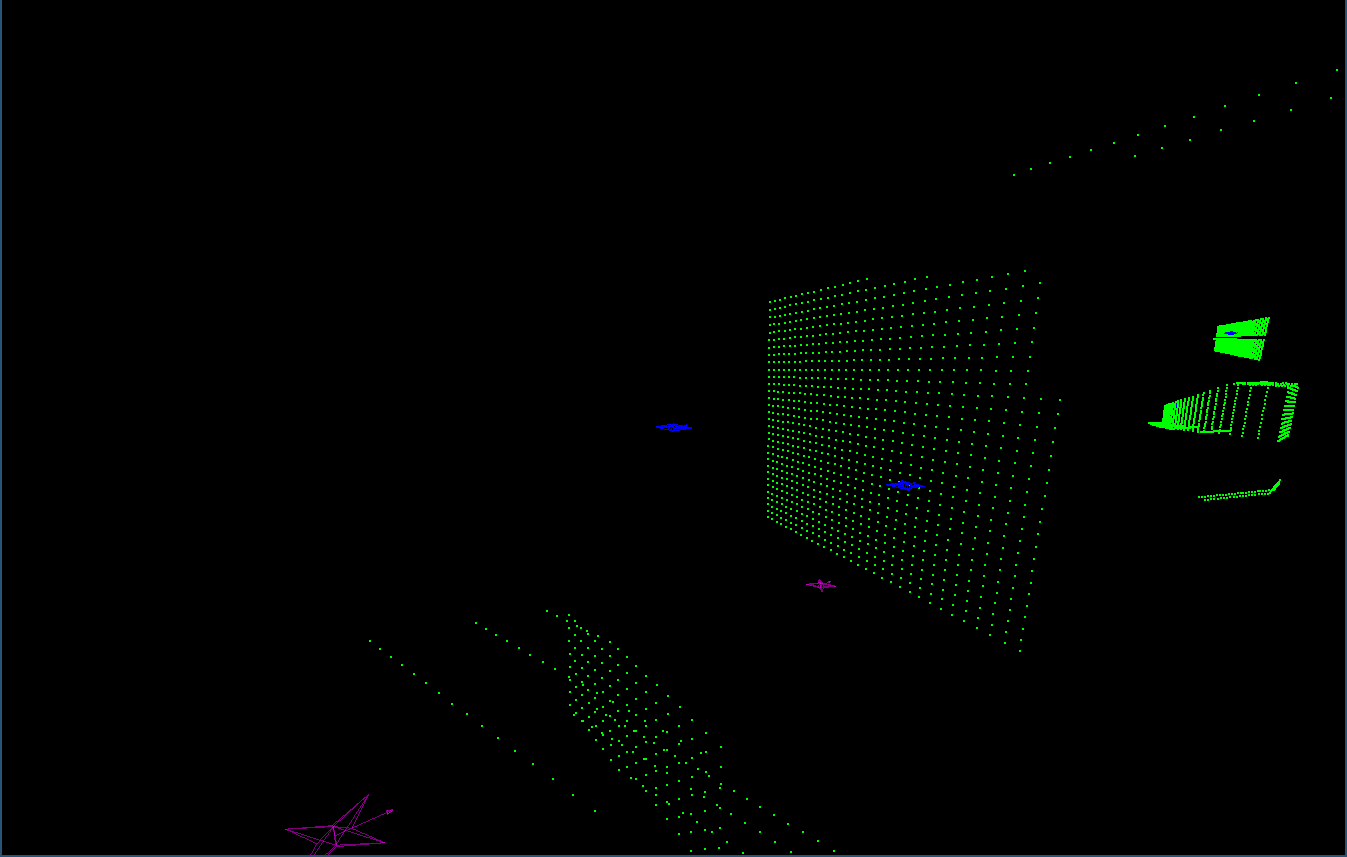
\includegraphics[width=0.33\linewidth]{units_dots1.png}
    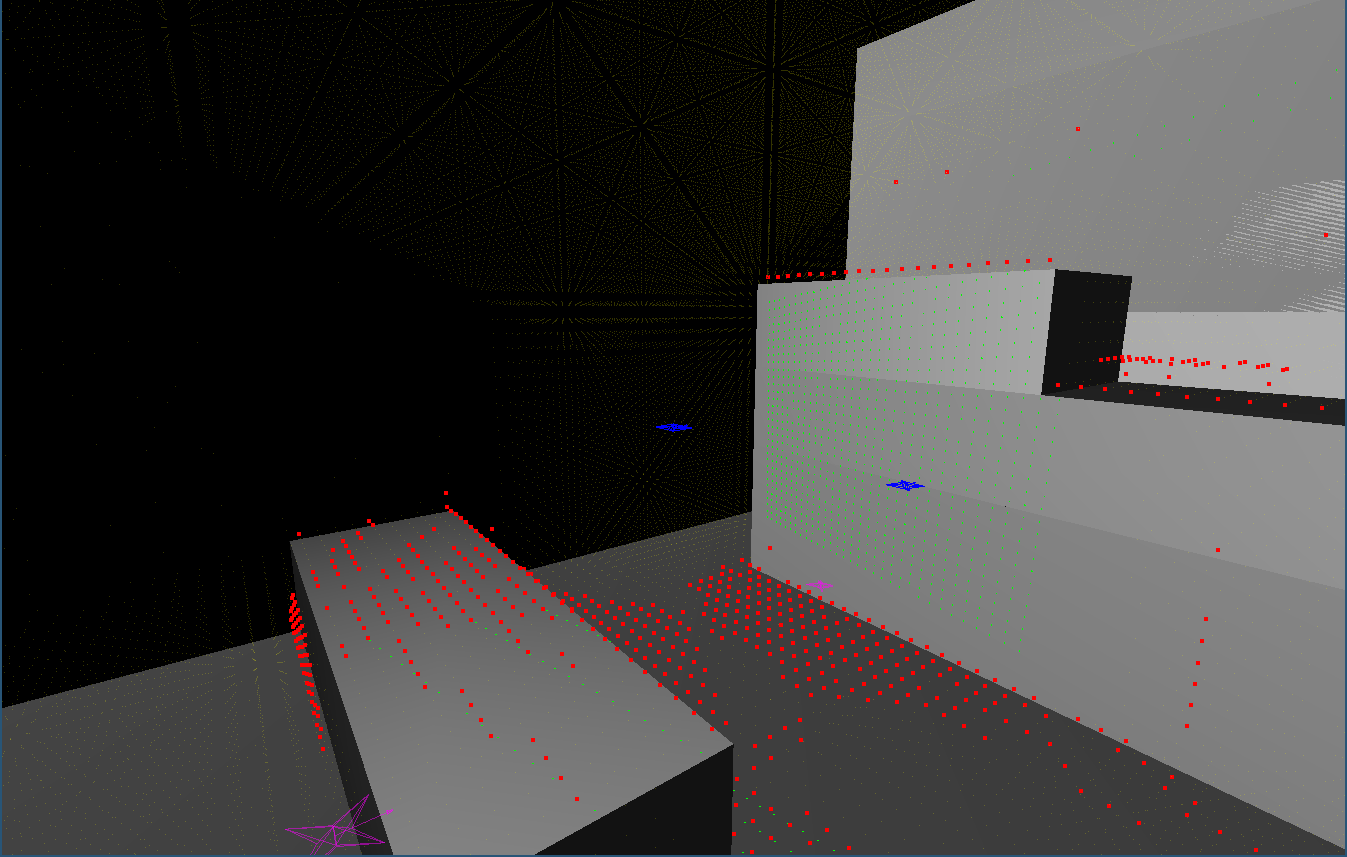
\includegraphics[width=0.33\linewidth]{all1.png}
\end{slide}

\begin{slide}

    \makeatletter
    \let\@topfil\relax
    \makeatother

    \textbf{Модель единицы массива}
    
    За основу была взята концепция БПЛА с вертикальным взлётом
    (коптер или вертолёт), тоесть юнит имеет возможность зависать в точке и резко изменять направление движения.
    Назовём единицу массива юнитом. Предполагается что каждый юнит имеет возможность
    оценить дальность в любом направлении, в нескольких точках одновременно с определённым 
    угловым разрешением (карта глубин). Также предполагается, что каждый юнит знает точно положение и скорость
    свои и остальных юнитов в массиве.

\end{slide}

\begin{slide}

    \makeatletter
    \let\@topfil\relax
    \makeatother

    \textbf{Заполнение карты}

    Каждый юнит получает информацю о мире с помощью датчика глубины в виде картинки,
    где каждому пикселю соответствует измерение дальности в определённых угловых координатах. В работе не эмулировлись
    дистрозийные искажения, поэтому для приведения карты глубин в точки в системе координат юнита достаточно 
    матрицы перспективной трансформации, которая имеется у каждого юнита. Она так же может меняться в процессе работы
    системы при необходимости (изменение угла обзора, зум). После получения точек в связанной системе координат они приводятся
    сначала к мировой, затем к системе координат карты. Так же приводится положение юнита (камеры) к системе координат карты.
    Заполняется карта по следующему алгоритму: строится отрезок из точки камеры к точке, полученной с датчика, все сектора, которые
    находятся между помечаются как исследованные, сектор, в котором находится точка с датчика помечается как заполненая.

\end{slide}

\begin{slide}

    \makeatletter
    \let\@topfil\relax
    \makeatother

    \textbf{Логика перемещения юнитов}

    Для системы в целом ставится задача полностью исследовать объём, отражаемый в карте.
    \begin{wrapfigure}[5]{r}{0.5\linewidth}
        \begin{center}
       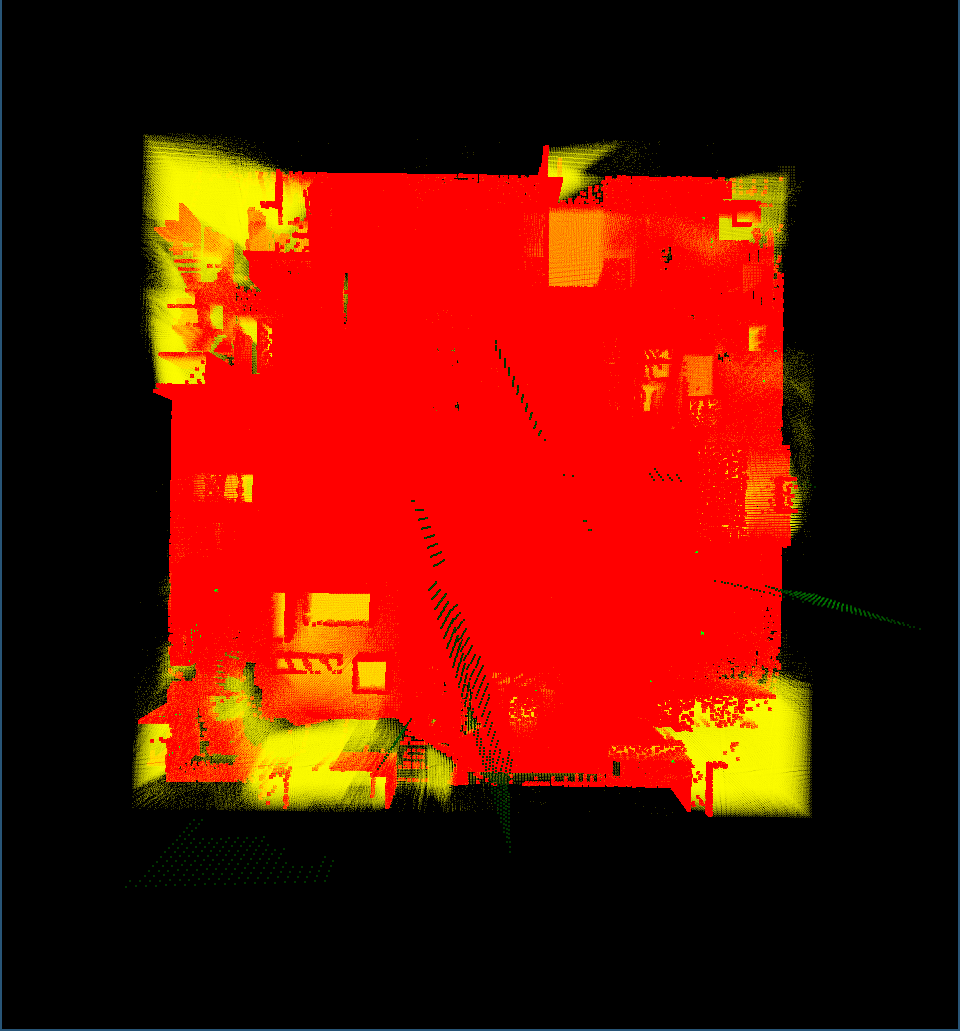
\includegraphics[width=0.8\linewidth]{pic1.png}
        \end{center}
    \end{wrapfigure}
    Из этого следует что каждый юнит направляется к ближайшему неизведанному участку. 
    На рисунке можно видеть жёлтые области -- эти области не обошёл сенсором ни один юнит.

\end{slide}

\begin{slide}

    \makeatletter
    \let\@topfil\relax
    \makeatother

    \textbf{Алгоритм перемещения юнитов}
    
    Важно чтобы юниты не сталкивались друг с другом и не врезались в стены.
    Для этого предусмотрены 2 алгоритма коррекции направления движения юнита: 
    \begin{mintemize}
        \item каждый юнит проверяет все остальные на предмет сближения и пересечения моментальной траектории
              (луч из юнита в направлении перемещения)
        \item происходит обращение к карте в целях получения ближайших заполненных секторов
    \end{mintemize}

\end{slide}

\begin{slide}

    \makeatletter
    \let\@topfil\relax
    \makeatother

    \textbf{Выводы}

    Тема малоизучена, но весьма перспективна и интересна. 
    Есть разрозненные наработки из других сфер, напрмер: 
    задачи трёхмерного сканирования объектов,
    системы технического зрения и т.д.

\end{slide}

\begin{slide}

    \makeatletter
    \let\@topfil\relax
    \makeatother

    \textbf{Дальнейшее направление работы}

    \begin{mintemize}
        \item доработать модель карты, чтобы иметь возможность охватывать непрямоугольные участки местности
        \item доработать модель карты, чтобы иметь разную детализацию в разных областях
        \item дополнить логику перемещения юнитов, с целью обеспечения полной радиосвязанности
        \item доработать модель карты, для хранения дополнительной информации (наличие движения, информация с тепловизоров)
        \item доработать алгоритм заполнения карты, возможно имеет смысл перерабатывать точки, поспупаемые с юнитов в 
                поверхности, так как это занимает меньше памяти и расширяет возможности для построения алгоритма обхода карты
        \item в связи с предидущим пунком дополнить алгоритм движения юнита (вдоль поверхности, на определённом расстоянии),
              это позволит лучше обследовать территорию
    \end{mintemize}

\end{slide}

\begin{cslide}
    \LARGE Спасибо за внимание.
\end{cslide}

\end{document}
